%%%%%%%%%%%%%%%%%%%%%%%%%%%%%%%%%%%%%%%%%%%%%%%%%%%%%%%%%%%%%%%%%
%  _____       ______   ____																		%
% |_   _|     |  ____|/ ____| 		Institute of Embedded Systems												%
%   | |  _ __ | |__  | (___    		Wireless Group														%
%   | | | '_ \|  __|  \___ \   		          Zuercher Hochschule Winterthur												%
%  _| |_| | | | |____ ____) |  		(University of Applied Sciences)												%
% |_____|_| |_|______|_____/  		8401 Winterthur, Switzerland												%
%																						%
%%%%%%%%%%%%%%%%%%%%%%%%%%%%%%%%%%%%%%%%%%%%%%%%%%%%%%%%%%%%%%%%%


% The ZHAW INES latex style scrip
\documentclass{clsFile/zhawines}


%INclude your own packages that are needed for you document, here the packages for the example are added
\usepackage{scrpage2}
\usepackage{listings}
\usepackage{amsmath}
\usepackage[squaren]{SIunits}
\usepackage{graphicx}
\usepackage{array}
\usepackage{float}

\begin{document}

%How the hyperlinks are shown, remove this or change it if you want the colorful links
\hypersetup{
    colorlinks = false,
    urlbordercolor = {1 1 1},
    linkbordercolor = {white},
}

%Select language, all generated content will be in the selected language
\selectlanguage{german} %possible german/english

% Generate your title page, it takes the arguments author, title
% and email. The title page is then generated with maketitle
\author{Autor1 \newline Autor2}
\title{Latex Vorlage}
\email{author@zhaw.ch}
\newcommand{\version}{0.1}

% Add Copyright informations and Contact infos
\newcommand{\confidential}{yes}  %write yes to have a confidential mark on every normal page

\maketitle


% Generate the header and footer of the document
\headings

%Include table of content
\tableofcontents

% Starts the page count from here, pdf viewers will be able to jump to the corret page.
 \setcounter{page}{1}

%Include all chapters. Chapters itself are in the content subfolder
%%%%%%%%%%%%%%%%%%%%%%%%%%%%%%%%%%%%%%%%%%%%%%%%%%%%%%%%%%%%%%%%%
%  _____       ______   ____									%
% |_   _|     |  ____|/ ____|  Institute of Embedded Systems	%
%   | |  _ __ | |__  | (___    Wireless Group					%
%   | | | '_ \|  __|  \___ \   Zuercher Hochschule Winterthur	%
%  _| |_| | | | |____ ____) |  (University of Applied Sciences)	%
% |_____|_| |_|______|_____/   8401 Winterthur, Switzerland		%
%																%
%%%%%%%%%%%%%%%%%%%%%%%%%%%%%%%%%%%%%%%%%%%%%%%%%%%%%%%%%%%%%%%%%

\chapter{LaTeX Kurzanleitung}\label{chap.anleitung}
Dieses Kapitel führt mit Beispielcode in den LaTeX Code ein, und kann während der Erstellung des Dokuments gelöscht werden.\footnote{Verbesserungsvorschläge bitte an hegt@zhaw.ch senden}

Die nachfolgende Berichtstruktur wurde aus der Vorlage\footnote{Berichtstruktur Vorlage, Stand: August 2011} der \href{https://intra.zhaw.ch/departemente/school-of-engineering/studium-standort-winterthur/studierende/projektarbeit-bachelorarbeit.html}{PA/BA Termin-Webseite} vom ZHAW Intranet entnommen.

(): alle in Klammer aufgeführten Einträge sind situativ anzupassen



Das ist ein kleiner Text um zu zeigen, wie die Enter eingebracht werden.\\
Ich finde Latex schwierig.\\
Der Start ist echt eine Herausforderung. \\
Mensch ist das Komplex, echt was für Profis. % Hier brauchts ja kein Enter mehr, sonnst heisst es Overfull \hbox



\section{Visio Vektorgraphik einfügen}\label{visio}
(Graphik auswählen) Speichern unter -> PDF -> Optionen.. -> Auswahl\\
Mit Adobe Akrobat öffnen: Erweitert -> Druckproduktion -> Seiten beschneiden -> Weisse Ränder entfernen -> OK -> Ctrl-S

\begin{figure}[H]
	\centering
		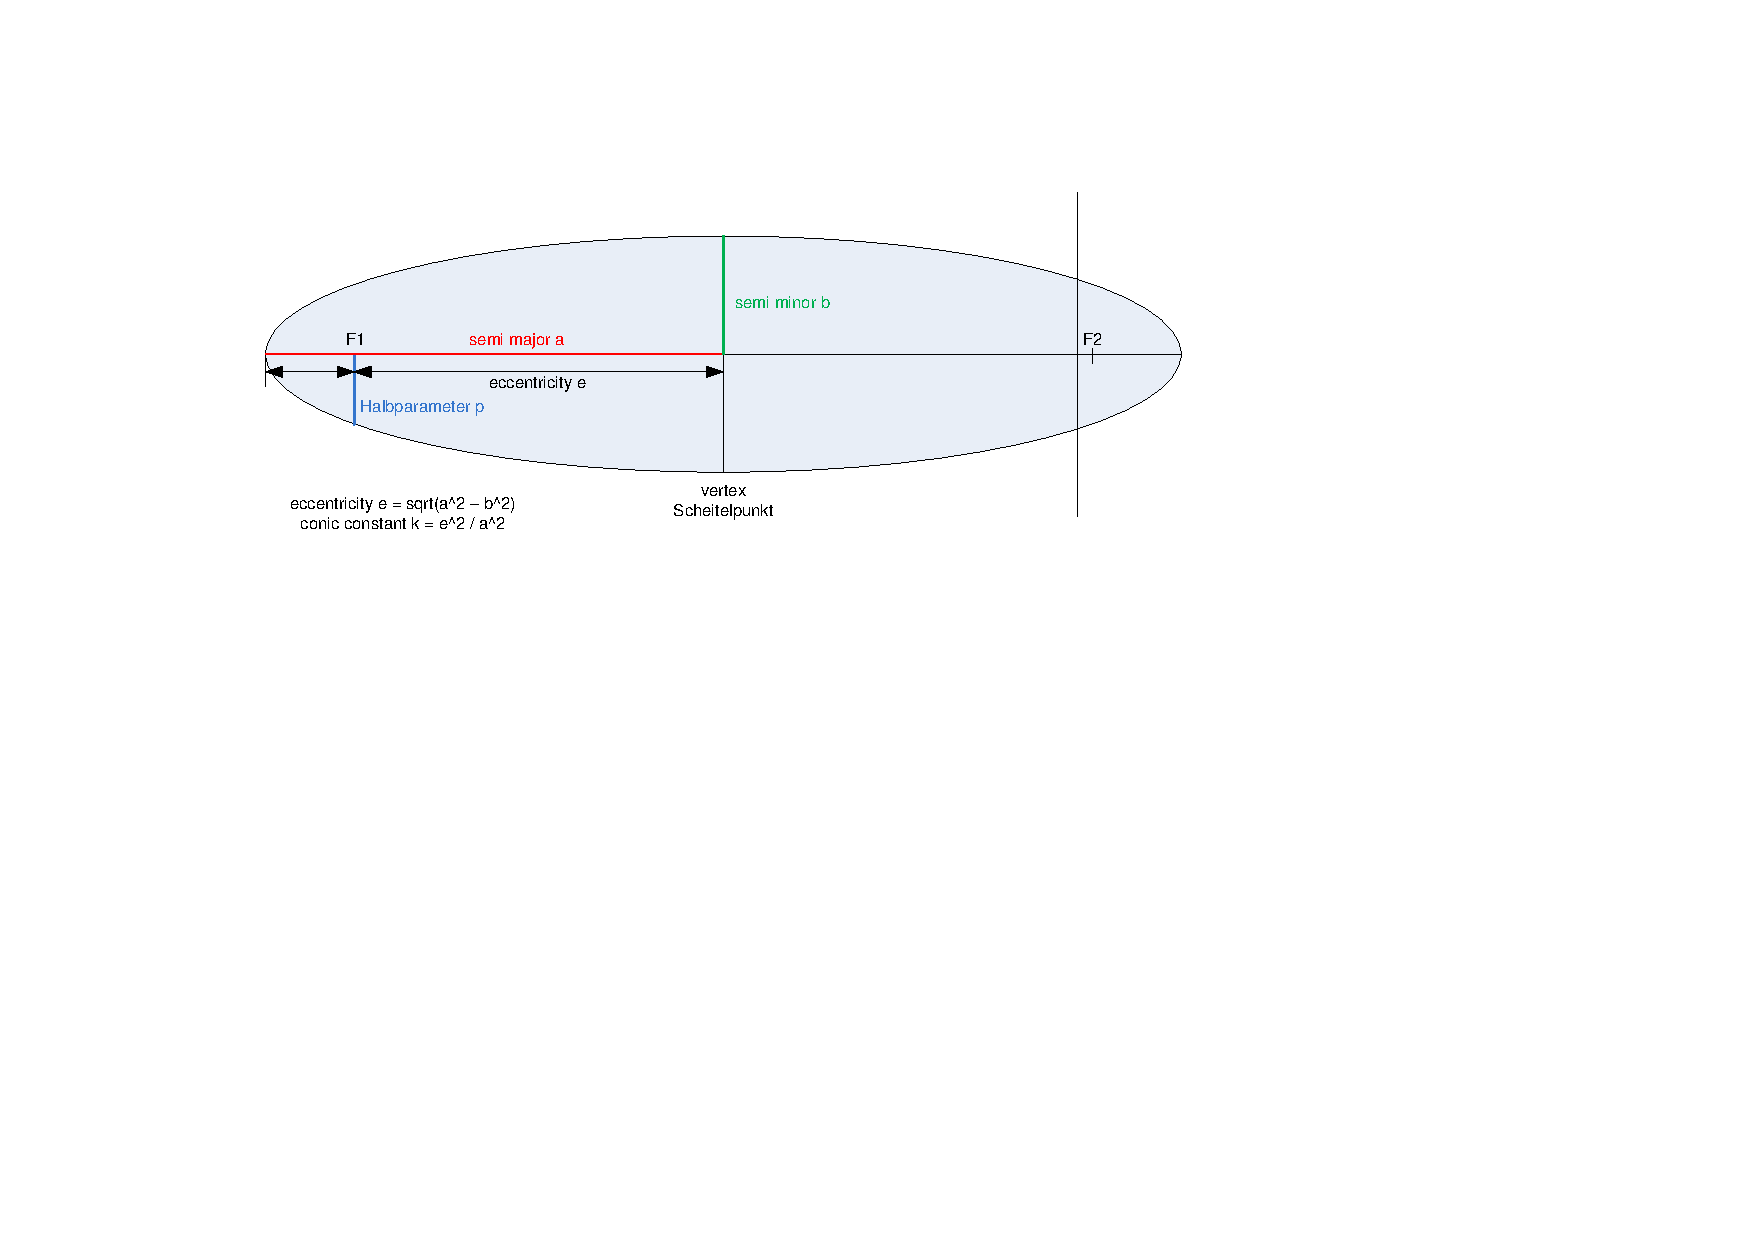
\includegraphics[width=0.8\textwidth]{images/visio/visio.pdf}
	\caption{Ideenskizze}
	\label{fig.Skizze}
\end{figure}

So kann die Abbildung~\ref{fig.Skizze} referenziert werden. Bei der PDF Erstellung ist darauf zu achten, dass LaTeX nur Versionen bis 1.4 voll unterstützt. 



\subsection{Graphiken in LaTeX zuschneiden}\label{zuschneiden}
Mit dem Befehl Clip kann eine Graphik auch in LaTeX zugeschnitten werden:

\begin{figure}[H]
	\centering
		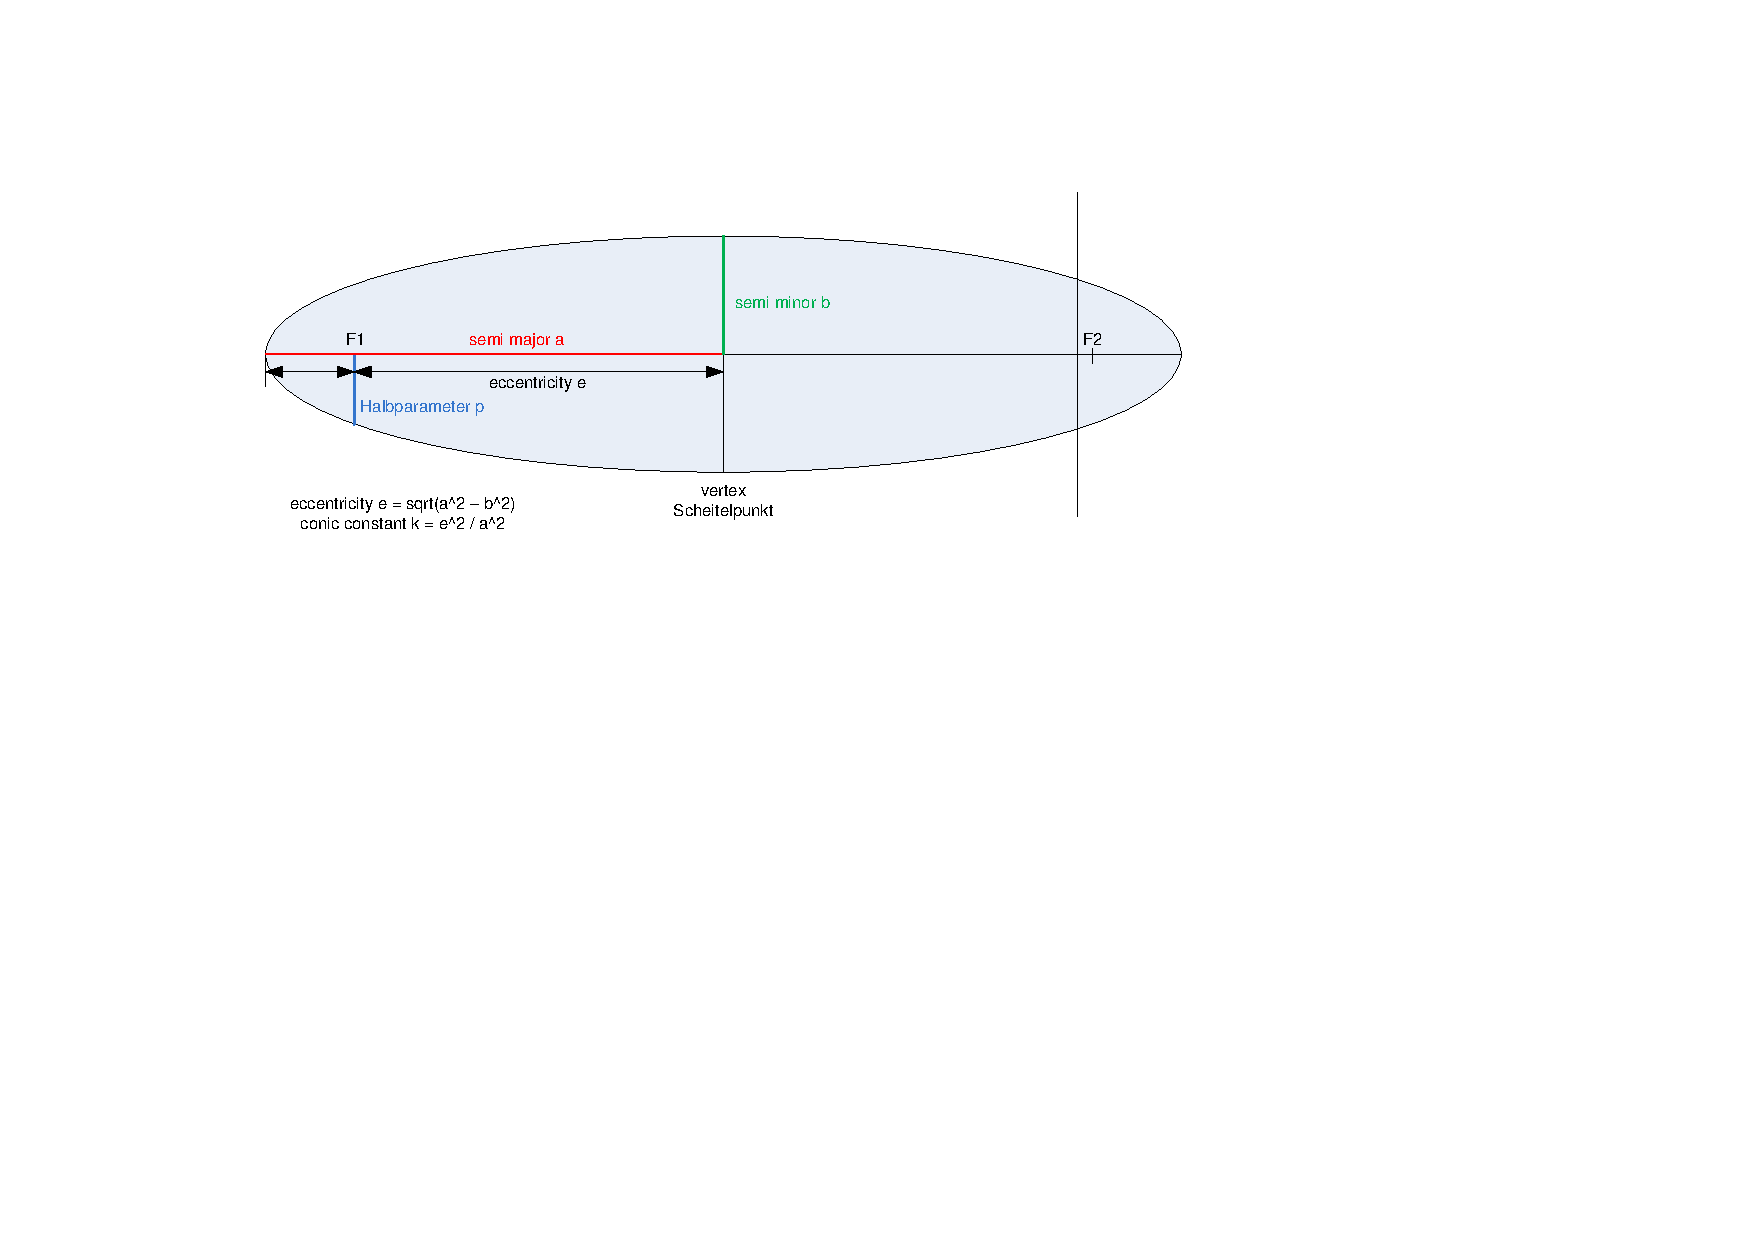
\includegraphics[width=0.9\textwidth, clip=true, trim = 80 10 0 10]{images/visio/visio.pdf}  % trim lm bm rm tm (left, bottom, right, top)
	\caption{clip=true, trim = 60 10 0 10}
	\label{fig.SkizzeZugeschnitten}
\end{figure}



\subsection{Mehrere Bilder nebeneinander}\label{nebeneinander}
Dank Minipages können mehrere Bilder auch nebeneinander sein:

%Zwei Bilder nebeneinander http://latex.mschroeder.net/
\begin{figure}[H]
  \centering
  \begin{minipage}[b]{0.45\textwidth}
    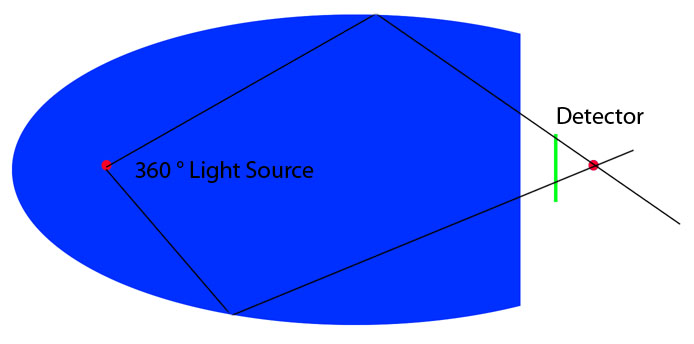
\includegraphics[scale=0.15]{images/photoshop/Skizze.jpg}
    \caption{Visir10b Detector}
    \label{Visir10bDetector} 
  \end{minipage} % Hier darf keine Leerzeile zwischen den beiden Minipages liegen!
  \begin{minipage}[b]{0.45\textwidth}
    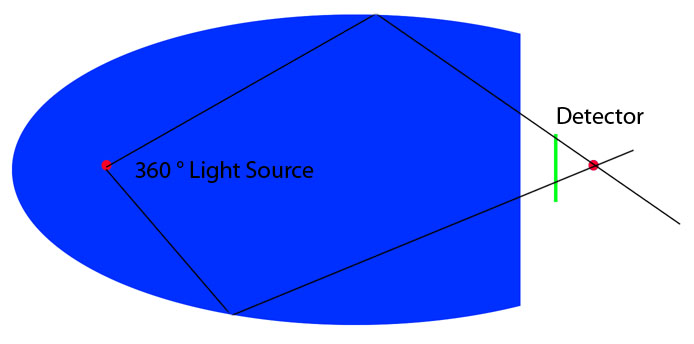
\includegraphics[scale=0.15]{images/photoshop/Skizze.jpg} 
    \caption{Visir10b Model}
    \label{Visir10bModel} 
  \end{minipage}
  \caption{Visir 10 mit optimiertem Reflektor}
  \label{fig.Visir10b}
\end{figure}


Literaturverweis: \citep{analog_devices_dac} \citep{microchip_spi}

\section{Tabellen aufbauen}\label{tabelle}
Kleine Tabelle:

\begin{table}[ht] \centering
	\begin{tabular}{|p{3cm}|p{.5cm}|p{.5cm}|p{.5cm}|p{.5cm}|p{.5cm}|p{.5cm}|p{.5cm}|p{.5cm}|p{.5cm}|p{.5cm}|} \hline
		\rowcolor{gray} Modul & M01 & M02 & M03 & M04 & M05 & M06 & M07 & M08 & M09 & M10 \\
		\hline
		FPGA\_DATEN & & & & & X & X & & X & X & \\
		\hline
		IRQ & X & X & X & & X & & & & X & X \\
		\hline
		Nachbar Core & & & & X & & X & & X & & \\
		\hline
	\end{tabular}
	\caption{Port Schwierigkeiten der Funkmodule}
	\label{tab:portprobleme}
 \end{table}	

Die nachfolgende longtable kann sich über mehrere Seiten erstrecken.

\begin{longtable}{|p{1.1cm}|p{4cm}|p{4cm}|p{4cm}|} 
					\hline
					\rowcolor{gray} Typ & Variante A & Variante B & Variante C
					\\ \hline
					& \textbf{Vorteile:} 
							\begin{itemize}
								\item[+] hohe Spannungen
							\end{itemize}							
							\textbf{Nachteile:}
							\begin{itemize}
								\item[-] Grosse Abmessung
							\end{itemize}
					& 	\textbf{Vorteile:} 
							\begin{itemize}
								\item[+] einfache Montage
							\end{itemize}							
							\textbf{Nachteile:}
							\begin{itemize}
								\item[-] max. 2A Eingangsstrom
							\end{itemize}
					&	\textbf{Vorteile:} 
							\begin{itemize}
								\item[+] hoher Strom
							\end{itemize}							
							\textbf{Nachteile:}
							\begin{itemize}
								\item[-] max. 12 V Eingangsspannung
							\end{itemize}\\ \hline
						Zeit & 2 h & 5 h & 3 h \\ \hline
						Preis	& 520 CHF/Stück & 800 CHF/Stück &	360 CHF/Stück\\ \hline
				\caption{Morphologischer Kasten für die Speisung}
				\label{tab:morphkasten}
			\end{longtable}	

Diese Art von Tabelle erstreckt sich immer auf der ganzen Seitenlänge:

\begin{tabularx}{\textwidth}{XXl}
  Salat & Schnecke & Igel\\
  Montag & Hier ist ein langes Wort & Dienstag
\end{tabularx}



\section{Code Listings aufbauen}\label{listing}

\begin{lstlisting}[
    language=C++,
    caption={Test Kommandozeilen Ausgabe},
    label={list.Testoutput}
]
/********************************************************/
/* Name        : M07Setup                               */
/* Description : EM9201 init for adress and pck         */
/* Input       : targetadr (DevAdr_M00 - DevAdr_M39)    */
/*               drate (Drate_M00 - Drate_M39)          */
/* Ouput       : -0x01 -> Setup OK                      */
/*               -0x5E -> Setup Error Channel write     */
/*               -0x6E -> Setup Error power write       */
/*               -0x7E -> Error in Device Address       */
/*               -0x8E -> Error in Peer Address         */
/********************************************************/
\end{lstlisting}

Formula $e = \sqrt{a{^2} - b^{2}}$


Diese Textstelle ist sehr interessant.\label{interessant}\\
Hier wird auf die Textstelle~\ref{interessant} verwiesen, die sich auf der Seite~\pageref{interessant} befindet.


% nogo:
% \ref{src:miktex} (\nameref{src:miktex})



\section{Citation nach IEEE}\label{citation}

Das ist ein \cite{robotvision} Verweis aufs Literaturverzeichnis. Ein anderes Beispiel ist das hier \cite{randompatterns}.





Das ist eine Aufzählung:
\begin{itemize} %
	\item Erste Zeile
	\item Zweite Zeile
	\item Dritte Zeile
\end{itemize}


\begin{enumerate}
\item erstens
\item zweitens
\end{enumerate}

%https://parma.zhaw.ch/svn/zhw_latex/
%gmanstyle nötig unter start od begin einbinden


Das ist eine verschachtelte Aufzählung:
\begin{description}
		\item [Register Performance] Alle Signale die das FPGA nicht verlassen, also von FF zu FF weitergeleitet werden. Daraus ergibt sich die maximale Taktfrequenz F\textsubscript{MAX}.

		\item [Externes Timing] FPGA Ein- und Ausgänge
		\begin{itemize}
			\item Ausgänge = Von FF's durch Logik zu Ausgängen (t\textsubscript{CO})
			\item Eingänge = Von Eingängen durch Logik zu FF's (t\textsubscript{SU}, t\textsubscript{H})
			\item Durchgänge = kombinatorische Pfade durch das FPGA (t\textsubscript{PD})
		\end{itemize}
\end{description}
 % Für das Schlussdokument auskommentieren
%%%%%%%%%%%%%%%%%%%%%%%%%%%%%%%%%%%%%%%%%%%%%%%%%%%%%%%%%%%%%%%%%
%  _____       ______   ____									%
% |_   _|     |  ____|/ ____|  Institute of Embedded Systems	%
%   | |  _ __ | |__  | (___    Wireless Group					%
%   | | | '_ \|  __|  \___ \   Zuercher Hochschule Winterthur	%
%  _| |_| | | | |____ ____) |  (University of Applied Sciences)	%
% |_____|_| |_|______|_____/   8401 Winterthur, Switzerland		%
%																%
%%%%%%%%%%%%%%%%%%%%%%%%%%%%%%%%%%%%%%%%%%%%%%%%%%%%%%%%%%%%%%%%%

\chapter{Einleitung}\label{chap.einleitung}


\section{Ausgangslage}\label{ausgangslage}

\begin{itemize}
\item Nennt bestehende Arbeiten/Literatur zum Thema -> Literaturrecherche
\item Stand der Technik: Bisherige Lösungen des Problems und deren Grenzen
\item (Nennt kurz den Industriepartner und/oder weitere Kooperationspartner und dessen/deren Interesse am Thema Fragestellung)
\end{itemize}



\section{Zielsetzung / Aufgabenstellung / Anforderungen}\label{zielsetzung}

\begin{itemize}
\item Formuliert das Ziel der Arbeit
\item Verweist auf die offizielle Aufgabenstellung des/der Dozierenden im Anhang
\item (Pflichtenheft, Spezifikation)
\item (Spezifiziert die Anforderungen an das Resultat der Arbeit)
\item (Übersicht über die Arbeit: stellt die folgenden Teile der Arbeit kurz vor)
\item (Angaben zum Zielpublikum: nennt das für die Arbeit vorausgesetzte Wissen)
\item (Terminologie: Definiert die in der Arbeit verwendeten Begriffe)
\end{itemize}

%%%%%%%%%%%%%%%%%%%%%%%%%%%%%%%%%%%%%%%%%%%%%%%%%%%%%%%%%%%%%%%%%
%  _____       ______   ____									%
% |_   _|     |  ____|/ ____|  Institute of Embedded Systems	%
%   | |  _ __ | |__  | (___    Wireless Group					%
%   | | | '_ \|  __|  \___ \   Zuercher Hochschule Winterthur	%
%  _| |_| | | | |____ ____) |  (University of Applied Sciences)	%
% |_____|_| |_|______|_____/   8401 Winterthur, Switzerland		%
%																%
%%%%%%%%%%%%%%%%%%%%%%%%%%%%%%%%%%%%%%%%%%%%%%%%%%%%%%%%%%%%%%%%%

\chapter{(Theoretische Grundlagen)}\label{chap.grundlagen}
 % (2. Theoretische Grundlagen)
%%%%%%%%%%%%%%%%%%%%%%%%%%%%%%%%%%%%%%%%%%%%%%%%%%%%%%%%%%%%%%%%%
%  _____       ______   ____									%
% |_   _|     |  ____|/ ____|  Institute of Embedded Systems	%
%   | |  _ __ | |__  | (___    Wireless Group					%
%   | | | '_ \|  __|  \___ \   Zuercher Hochschule Winterthur	%
%  _| |_| | | | |____ ____) |  (University of Applied Sciences)	%
% |_____|_| |_|______|_____/   8401 Winterthur, Switzerland		%
%																%
%%%%%%%%%%%%%%%%%%%%%%%%%%%%%%%%%%%%%%%%%%%%%%%%%%%%%%%%%%%%%%%%%

\chapter{Vorgehen / Methoden}\label{chap.vorgehen}


\begin{itemize}
\item (Beschreibt die Grundüberlegungen der realisierten Lösung (Konstruktion/Entwurf) und die Realisierung als Simulation, als Prototyp oder als Software-Komponente)
\item (Definiert Messgrössen, beschreibt Mess- oder Versuchsaufbau, beschreibt und dokumentiert Durchführung der Messungen/Versuche)
\item (Experimente)
\item (Lösungsweg)
\item (Modell)
\item (Tests und Validierung)
\item (Theoretische Herleitung der Lösung)
\end{itemize}



\section{(Verwendete Software)}\label{software}
Für die vorliegende Arbeit wurden die unten aufgeführten Programme eingesetzt.

\subsection*{Arbeitsumgebung}\label{wintool}
\begin{itemize}
	\item Microsoft Windows 8 developer preview
\end{itemize}

\subsection*{Virtual Machine}\label{vm}
\begin{itemize}
	\item Oracle VM VirtualBox, Version 3.2.10
\end{itemize}

\subsection*{CAD Catia}\label{catia}
\begin{itemize}
	\item CATIA, Version 5.19 (in VirtualBox)
\end{itemize}

\subsection*{Dokumentation}\label{dokutools}
\begin{itemize}
	\item proTeXt mit TexMakerX 2.1 (SVN 1774), \href{http://www.latex-project.org/ftp.html}{latex-project.org}
	\item Microsoft Visio 2007
	\item Adobe Acrobat 8 Professional 8.1.6
\end{itemize}
 % Vorgehen / Methoden
%%%%%%%%%%%%%%%%%%%%%%%%%%%%%%%%%%%%%%%%%%%%%%%%%%%%%%%%%%%%%%%%%
%  _____       ______   ____									%
% |_   _|     |  ____|/ ____|  Institute of Embedded Systems	%
%   | |  _ __ | |__  | (___    Wireless Group					%
%   | | | '_ \|  __|  \___ \   Zuercher Hochschule Winterthur	%
%  _| |_| | | | |____ ____) |  (University of Applied Sciences)	%
% |_____|_| |_|______|_____/   8401 Winterthur, Switzerland		%
%																%
%%%%%%%%%%%%%%%%%%%%%%%%%%%%%%%%%%%%%%%%%%%%%%%%%%%%%%%%%%%%%%%%%

\chapter{Resultate}\label{chap.resultate} 

\begin{itemize}
\item (Zusammenfassung der Resultate)
\end{itemize}

%%%%%%%%%%%%%%%%%%%%%%%%%%%%%%%%%%%%%%%%%%%%%%%%%%%%%%%%%%%%%%%%%
%  _____       ______   ____									%
% |_   _|     |  ____|/ ____|  Institute of Embedded Systems	%
%   | |  _ __ | |__  | (___    Wireless Group					%
%   | | | '_ \|  __|  \___ \   Zuercher Hochschule Winterthur	%
%  _| |_| | | | |____ ____) |  (University of Applied Sciences)	%
% |_____|_| |_|______|_____/   8401 Winterthur, Switzerland		%
%																%
%%%%%%%%%%%%%%%%%%%%%%%%%%%%%%%%%%%%%%%%%%%%%%%%%%%%%%%%%%%%%%%%%

\chapter{Diskussion und Ausblick}\label{chap.diskussion}

\begin{itemize}
\item Bespricht die erzielten Ergebnisse bezüglich ihrer Erwartbarkeit, Aussagekraft und Relevanz
\item Interpretation und Validierung der Resultate
\item Rückblick auf Aufgabenstellung, erreicht bzw. nicht erreicht
\item Legt dar, wie an die Resultate (konkret vom Industriepartner oder weiteren Forschungsarbeiten; allgemein) angeschlossen werden kann; legt dar, welche Chancen die Resultate bieten
\end{itemize}
 % Diskussion und Ausblick


% Generate the bibliography and add it to the table of contents, there is an extra bib file where you can add entries(subfolder BibTeX-Literaturverzeichnis)
\addcontentsline{toc}{chapter}{\bibname}
\bibliographystyle{unsrt}
\bibliography{BibTex/literatur}

% Additional lists
\listoffigures
\listoftables
%%%%%%%%%%%%%%%%%%%%%%%%%%%%%%%%%%%%%%%%%%%%%%%%%%%%%%%%%%%%%%%%%
%  _____       ______   ____									%
% |_   _|     |  ____|/ ____|  Institute of Embedded Systems	%
%   | |  _ __ | |__  | (___    Wireless Group					%
%   | | | '_ \|  __|  \___ \   Zuercher Hochschule Winterthur	%
%  _| |_| | | | |____ ____) |  (University of Applied Sciences)	%
% |_____|_| |_|______|_____/   8401 Winterthur, Switzerland		%
%																%
%%%%%%%%%%%%%%%%%%%%%%%%%%%%%%%%%%%%%%%%%%%%%%%%%%%%%%%%%%%%%%%%%

\chapter*{Abkürzungsverzeichnis}\label{chap.glossar}
\addcontentsline{toc}{section}{(Abkürzungsverzeichnis)}\label{cha:abkürzungsverzeichnis}

In diesem Abschnitt werden Abkürzungen und Begriffe kurz erklärt.

\begin{longtable}{|m{3cm}|m{11cm}|}\hline	
	\rowcolor{gray} \textbf{Abk}&
	Abkürzung \\ \hline	

	\textbf{XY}&
	Ix Ypsilon \\ \hline	
	
	\textbf{YZ}&
	Ypsilon Zet \\ \hline
	
	
	
	
	
%\caption{Abkürzungs Verzeichnis}
%\label{tab:glossar}
\end{longtable}

\lstlistoflistings

%%%%%%%%%%%%%%%%%%%%%%%%%%%%%%%%%%%%%%%%%%%%%%%%%%%%%%%%%%%%%%%%%
%  _____       ______   ____									%
% |_   _|     |  ____|/ ____|  Institute of Embedded Systems	%
%   | |  _ __ | |__  | (___    Wireless Group					%
%   | | | '_ \|  __|  \___ \   Zuercher Hochschule Winterthur	%
%  _| |_| | | | |____ ____) |  (University of Applied Sciences)	%
% |_____|_| |_|______|_____/   8401 Winterthur, Switzerland		%
%																%
%%%%%%%%%%%%%%%%%%%%%%%%%%%%%%%%%%%%%%%%%%%%%%%%%%%%%%%%%%%%%%%%%


\pagenumbering{Roman}

\appendix
\chapter{Anhang}\label{chap.anhang}



\section{Projektmanagement}\label{projektmanagement}

\begin{itemize}
\item Offizielle Aufgabenstellung, Projektauftrag
\item (Zeitplan)
\item (Besprechungsprotokolle oder Journals)
\end{itemize}



\section{Weiteres}\label{weiteres}

\begin{itemize}
\item CD mit dem vollständigen Bericht als pdf-File inklusive Film- und Fotomaterial
\item (Schaltpläne und Ablaufschemata)
\item (Spezifikationen u. Datenblätter der verwendeten Messgeräte und/oder Komponenten)
\item (Berechnungen, Messwerte, Simulationsresultate)
\item (Stoffdaten)
\item (Fehlerrechnungen mit Messunsicherheiten)
\item (Grafische Darstellungen, Fotos)
\item (Datenträger mit weiteren Daten (z.B. Software-Komponenten) inkl. Verzeichnis der auf diesem Datenträger abgelegten Dateien)
\item (Softwarecode)
\end{itemize}
 % Anhang

\end{document}
